%% -*- latex -*-
%%%%%%%%%%%%%%%%%%%%%%%%%%%%%%%%%%%%%%%%%%%%%%%%%%%%%%%%%%%%%%%%
%%%%
%%%% This TeX file is part of the course
%%%% Introduction to Scientific Programming in C++/Fortran2003
%%%% copyright 2017-2023 Victor Eijkhout eijkhout@tacc.utexas.edu
%%%%
%%%% queens.tex : the classic `eight queens' problem
%%%%
%%%%%%%%%%%%%%%%%%%%%%%%%%%%%%%%%%%%%%%%%%%%%%%%%%%%%%%%%%%%%%%%

\begin{wrapfigure}{r}{3in}
  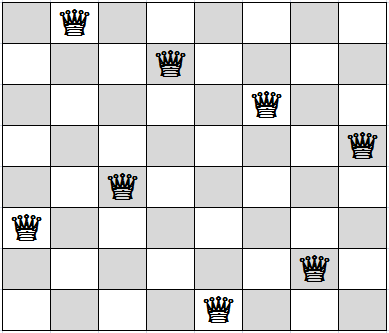
\includegraphics[scale=.75]{eightqueens}
\end{wrapfigure}
A famous exercise for recursive programming is the
\indexterm{eight queens} problem:
Is it possible to position eight queens on a chess board,
so that no two queens `threaten' each other,
according to the rules of chess?

\Level 0 {Problem statement}

The precise statement of the `eight queens problem' is:
\begin{itemize}
\item Put eight pieces on an $8\times8$ board, no two pieces on the same square; so that
\item no two pieces are on the same row,
\item no two pieces are on the same column, and
\item no two pieces are on the same diagonal.
\end{itemize}
A~systematic solution would run:
\begin{enumerate}
\item put a piece anywhere in the first row;
\item for each choice in the first row, try all positions in the second row;
\item for all choices in the first two rows, try all positions in the third row;
\item when you have a piece in all eight rows, evaluate the board to
  see if it satisfies the condition.
\end{enumerate}
\begin{exercise}
  This algorithm will generate all $8^8$ boards.
  Do you see at least one way to speed up the search?
\end{exercise}

Since the number eight is, for now, fixed, you could write this code
as an eight-deep loop nest. However that is not elegant.
For example, the only reason for the number~8 in the above exposition
is that this is the traditional size of a chess board.
The problem, stated more abstractly as placing $n$ queens on an $n\times n$ board,
has solutions for~$n\geq 4$.

\Level 0 {Solving the eight queens problem, basic approach}
\label{sec:8queens-strategy}

This problem requires you to know about arrays/vectors;
chapter~\textbookref{ch:array}.
Also, see chapter~\textbookref{ch:tdd} for \ac{TDD}.
Finally, see section~\textbookref{sec:std-optional} for \lstinline+std::optional+.

The basic strategy will be that we fill consecutive rows,
by indicating each time which column will be occupied by the next queen.
Using an \ac{OO} strategy, we make a class \lstinline{ChessBoard},
that holds a partially filled board.

The basic solution strategy is recursive:
\begin{itemize}
\item Let \lstinline{current} be the current, partially filled board;
\item We call \lstinline{current.place_queens()} that tries to finish the board;
\item However, with recursion, this method only fills one row,
  and then calls \lstinline+place_queens+ on this new board.
\end{itemize}
So
\begin{lstlisting}
ChessBoard::place_queens() {
  // for c = 1 ... number of columns:
  //   make a copy of the board
  //   put a queen in the next row, column c, of the copy
  //   and call place_queens() on that copy;
  //   investigate the result.....
}
\end{lstlisting}
This routine returns either a solution, or an indication that no solution was possible.

In the next section we will develop a solution
systematically in a \ac{TDD} manner.

\Level 0 {Developing a solution by TDD}
\label{sec:8queens-tdd}

We now gradually develop the \ac{OO} solution to the eight queens problem,
using test-driven development.

\heading{The board}

We start by constructing a board,
with a constructor that only indicates the size of the problem:
\verbatimsnippet{boardconstructorn}
This is a `generalized chess board' of size~$n\times n$,
and initially it should be empty.

\begin{exercise}
  Write this constructor, for an empty board of size~$n\times n$.
\end{exercise}

Note that the implementation of the board is totally up to you.
In the following you will get tests for functionality
that you need to satisfy, but any implementation that makes this true
is a correct solution.

\heading{Bookkeeping: what's the next row?}

Assuming that we fill in the board row-by-row,
we have an auxiliary function that returns  the next row to be filled:
\verbatimsnippet{boardnextloc}

This gives us our first simple test:
on an empty board, the row to be filled in is row~zero.

\begin{exercise}
  Write this method and make sure that it passes the test for an empty board.
  \verbatimsnippet{qtempty}
\end{exercise}

By the rules of \ac{TDD} you can actually write the method so that it only
satisfies the test for the empty board.
Later, we will test that this method gives the right result
after we have filled in a couple of rows,
and then of course your implementation needs to be general.

\heading{Place one queen}

Next, we have a function to place the next queen,
whether this gives a feasible board
(meaning that no pieces can capture each other) or not:
\verbatimsnippet{boardplacenext}

This method should first of all catch incorrect indexing:
we assume that the placement routine throws an exception
for invalid column numbers.
\begin{lstlisting}
ChessBoard::place_next_queen_at_column( int c ) {
  if ( /* c is outside the board */ )
    throw(1); // or some other exception.
\end{lstlisting}

(Suppose you didn't test for incorrect indexing.
Can you construct a simple `cheating' solution
at any size?)

\begin{exercise}
  Write this method, and make sure it passes the following test for
  valid and invalid column numbers:
  \verbatimsnippet{qtfillfirst}
  (From now on we'll only give the body of the test.)
\end{exercise}

Now it's time to start writing some serious stuff.

\heading{Is a (partial) board feasible?}

If you have a board,
even partial,
you want to test if it's feasible,
meaning that the queens that have been placed can not capture each other.

The prototype of this method is:
\verbatimsnippet{boardfeasibleproto}

This test has to work for simple cases to begin with:
an empty board is feasible, as is a board with only one piece.
\verbatimsnippet{qtfeasible0}
\verbatimsnippet{qtfeasible1}

\begin{exercise}
  Write the method and make sure it passes these tests.
\end{exercise}

We shouldn't only do successful tests,
sometimes referred to as the `happy path' through the code.
For instance,
if we put two queens in the same column, the test should fail.

\begin{exercise}
  Take the above initial attempt with a queen in position $(0,0)$,
  and add another queen in column zero of the next row.
  Check that it passes the test:
  \verbatimsnippet{qtcollide}
  Add a few tests more of your own.
  (These will not be exercised by the submission script,
  but you may find them useful anyway.)
\end{exercise}

\heading{Testing configurations}

If we want to test the feasibility of non-trivial configurations,
it is a good idea to be able to `create' solutions.
For this we need a second type of constructor
where we construct a fully filled chess board
from the locations of the pieces.
%
\verbatimsnippet{boardconstructorv}
\begin{itemize}
\item If the constructor is called with only a vector, this describes a full board.
\item Adding an integer parameter indicates the size of the board,
  and the vector describes only the rows that have been filled in.
\end{itemize}

\begin{exercise}
  Write these constructors, and
  test that an explicitly given solution is a feasible board:
  %
  \verbatimsnippet{qtsolution5}
\end{exercise}

For an elegant approach to implementing this,
see \indextermsub{delegating}{constructor}s;
section~\textbookref{sec:construct-delegate}.

Ultimately we have to write the tricky stuff.

\Level 0 {The recursive solution method}

The main function
\verbatimsnippet{queenplaceproto}
takes a board, empty or not, and tries to fill the remaining rows.

One problem is that this method needs to be able to communicate
that, given some initial configuration, no solution is possible.
For this, we let the return type of \lstinline+place_queens+
be \lstinline+optional<ChessBoard>+:
\begin{itemize}
\item if it is possible to finish the current board resulting in a solution,
  we return that filled board;
\item otherwise we return \lstinline+{}+, indicating that no solution was possible.
\end{itemize}

With the recursive strategy discussed in section~\ref{sec:8queens-strategy},
this placement method has roughly the following structure:
\begin{lstlisting}
place_queens() {
  for ( int col=0; col<n; col++ ) {
    ChessBoard next = *this;
    // put a queen in column col on the `next' board
    // if this is feasible and full, we have a solution
    // if it is feasible but no full, recurse
  }
}
\end{lstlisting}

The line
\begin{lstlisting}
ChessBoard next = *this;
\end{lstlisting}
makes a copy of the object you're in.

\begin{remark}
  Another approach would be to  make a recursive function
\begin{lstlisting}
bool place_queen( const ChessBoard& current, ChessBoard &next );
// true if possible, false is not
\end{lstlisting}
\end{remark}

\heading{The final step}

Above you coded the method \lstinline+feasible+
that tested whether a board is still a candidate for a solution.
Since this routine works for any partially filled board,
you also need a method to test if you're done.

\begin{exercise}
  Write a method
\begin{lstlisting}
bool filled();
\end{lstlisting}
  and write a test for it, both positive and negative.
\end{exercise}

Now that you can recognize solutions, it's time to
write the solution routine.
\begin{exercise}
  Write the method \verbatimsnippet{queenplaceproto}
\end{exercise}

Because the function \lstinline+place_queens+ is recursive,
it is a little hard to test in its entirety.

We start with a simpler test:
if you almost have the solution,
it can do the last step.

\begin{exercise}
  Use the constructor 
\begin{lstlisting}
ChessBoard( int n,vector<int> cols )
\end{lstlisting}
to generate a board that has all but the last row filled in,
and that is still feasible. Test that you can find the solution:
  \verbatimsnippet{qtfilllast}
\end{exercise}

Since this test only fills in the last row,
it only does one loop,
so printing out diagnostics is possible,
without getting overwhelmed in tons of output.

\heading{Solutions and non-solutions}

Now that you have the solution routine,
test that it works starting from an empty board.
For instance, confirm there are no $3\times 3$ solutions:
\verbatimsnippet{qtfail3x3}
On the other hand, $4\times4$ solutions do exist:
\verbatimsnippet{qtdo4x4}

\begin{exercise}
  (Optional) Can you modify your code so that it counts all the possible
  solutions?
\end{exercise}

\begin{exercise}
  (Optional) How does the time to solution behave as function of~$n$?
\end{exercise}

